\section{Les périphériques du
microcontrôleur}\label{les-puxe9riphuxe9riques-du-microcontruxf4leur}

\begin{frame}{Les périphériques du microcontrôleur}

\begin{center}
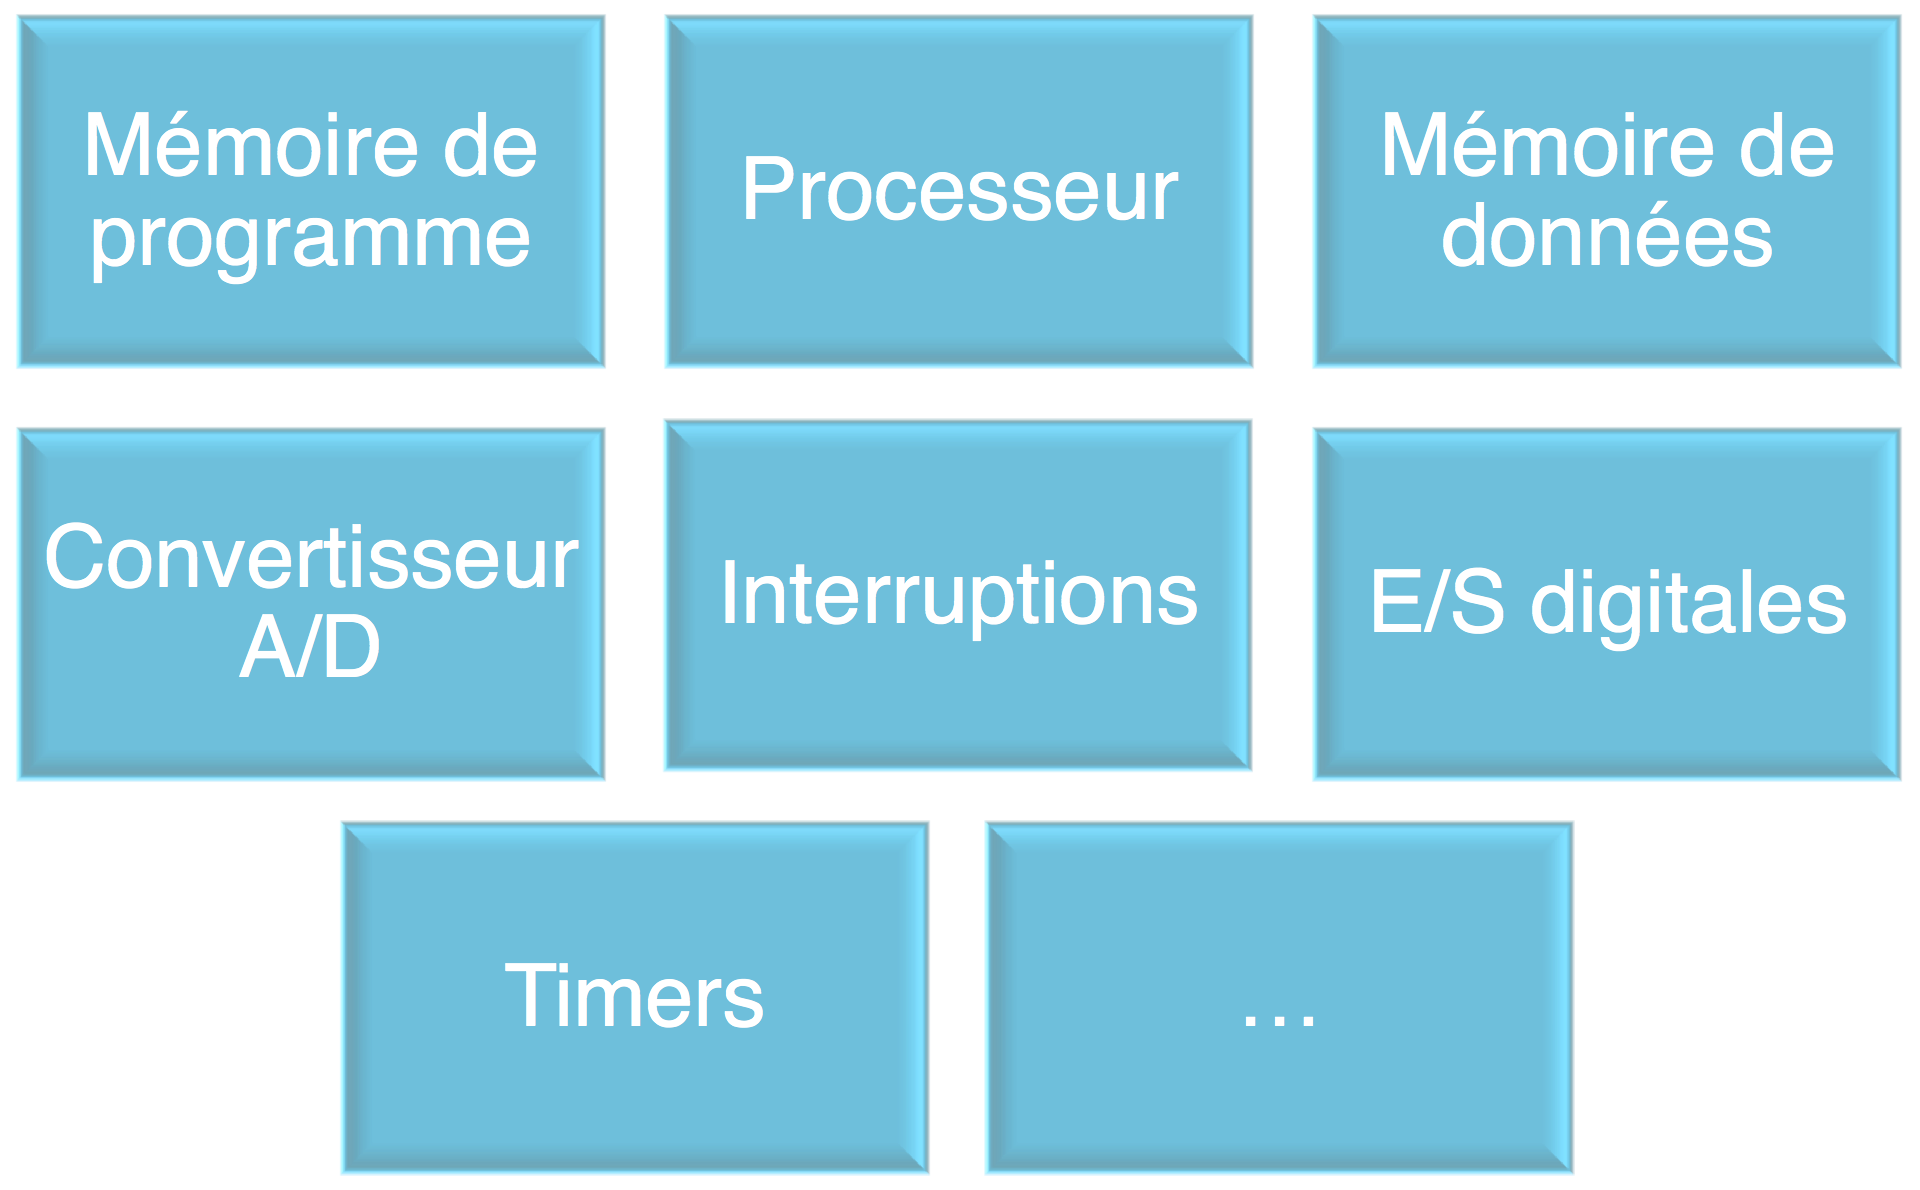
\includegraphics[width=.5\textwidth]{images/architecture.png}
\end{center}

\begin{itemize}
\itemsep1pt\parskip0pt\parsep0pt
\item
  La communication bidirectionnelle entre le processeur et ses
  périphériques se fait au travers de ``registres à fonctions
  spéciales'' = emplacements dans la mémoire qui ont une fonction
  particulière.
\item
  Ces registres à fonctions spéciales ont des noms pré-définis que l'on
  peut utiliser dans notre programme.
\end{itemize}

\end{frame}

\section{Entrées/sorties digitales}\label{entruxe9essorties-digitales}

\begin{frame}{Entrées/sorties digitales}

\begin{itemize}
\itemsep1pt\parskip0pt\parsep0pt
\item
  Un port d'E/S est un module qui contrôle 8 broches du microcontrôleur
\item
  La communication entre le module et le programme a lieu au travers de
  3 registres à fonctions spéciales

  \begin{itemize}
  \itemsep1pt\parskip0pt\parsep0pt
  \item
    TRIS{[}x{]} : direction (x : lettre du port)
  \item
    PORT{[}x{]} : lecture des pins
  \item
    LAT{[}x{]} : écriture d'un état logique
  \end{itemize}
\item
  Remarque : on peut accéder à un bit particulier de la manière suivante
  :

  \begin{itemize}
  \itemsep1pt\parskip0pt\parsep0pt
  \item
    LAT{[}x{]}bits.LAT{[}x{]}{[}n{]} (n : le numéro de la broche
    {[}0..7{]})
  \item
    PORT{[}x{]}bits.R{[}x{]}{[}n{]}
  \item
    TRIS{[}x{]}bits.TRIS{[}x{]}{[}n{]}
  \end{itemize}
\end{itemize}

\end{frame}

\begin{frame}{Entrées/sorties digitales, Exemples}

\begin{itemize}
\item
  getButton()\\Le bouton est connecté sur la broche 0 du port B
\item
  setLeds() Les LEDs sont connectées sur toutes les broches du port D
\item
  LATDbits.LATB1 = 1; \textless{}=\textgreater{} LATD \textbar{} 0x02;
\item
  LATDbits.LATB2 = 0; \textless{}=\textgreater{} LATD \& 0xFB;
\end{itemize}

\end{frame}

\section{Conversion
analogique-digital}\label{conversion-analogique-digital}

\begin{frame}{Conversion analogique-digital (1)}

\begin{center}
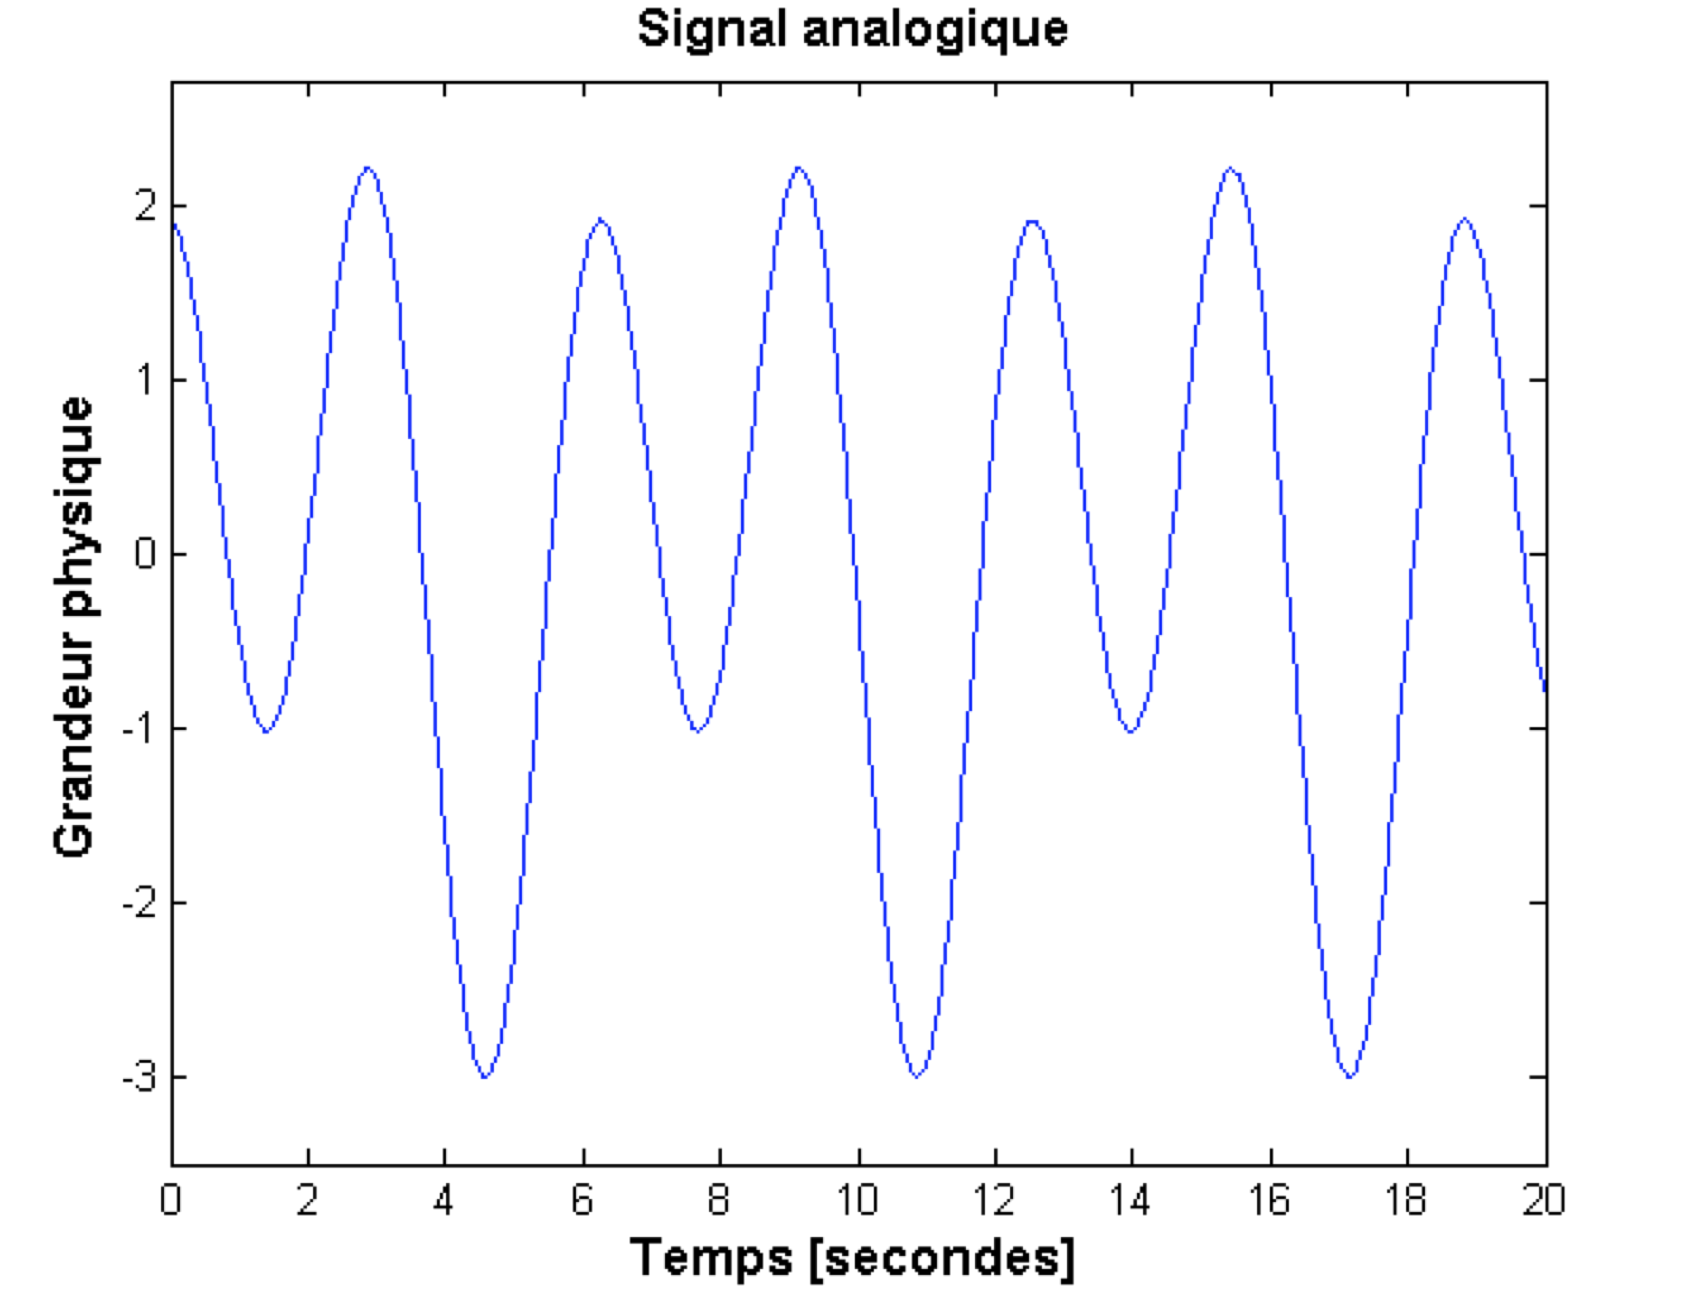
\includegraphics[width=.8\textwidth]{images/ad_0.png}
\end{center}

\end{frame}

\begin{frame}{Conversion analogique-digital (2)}

\begin{center}
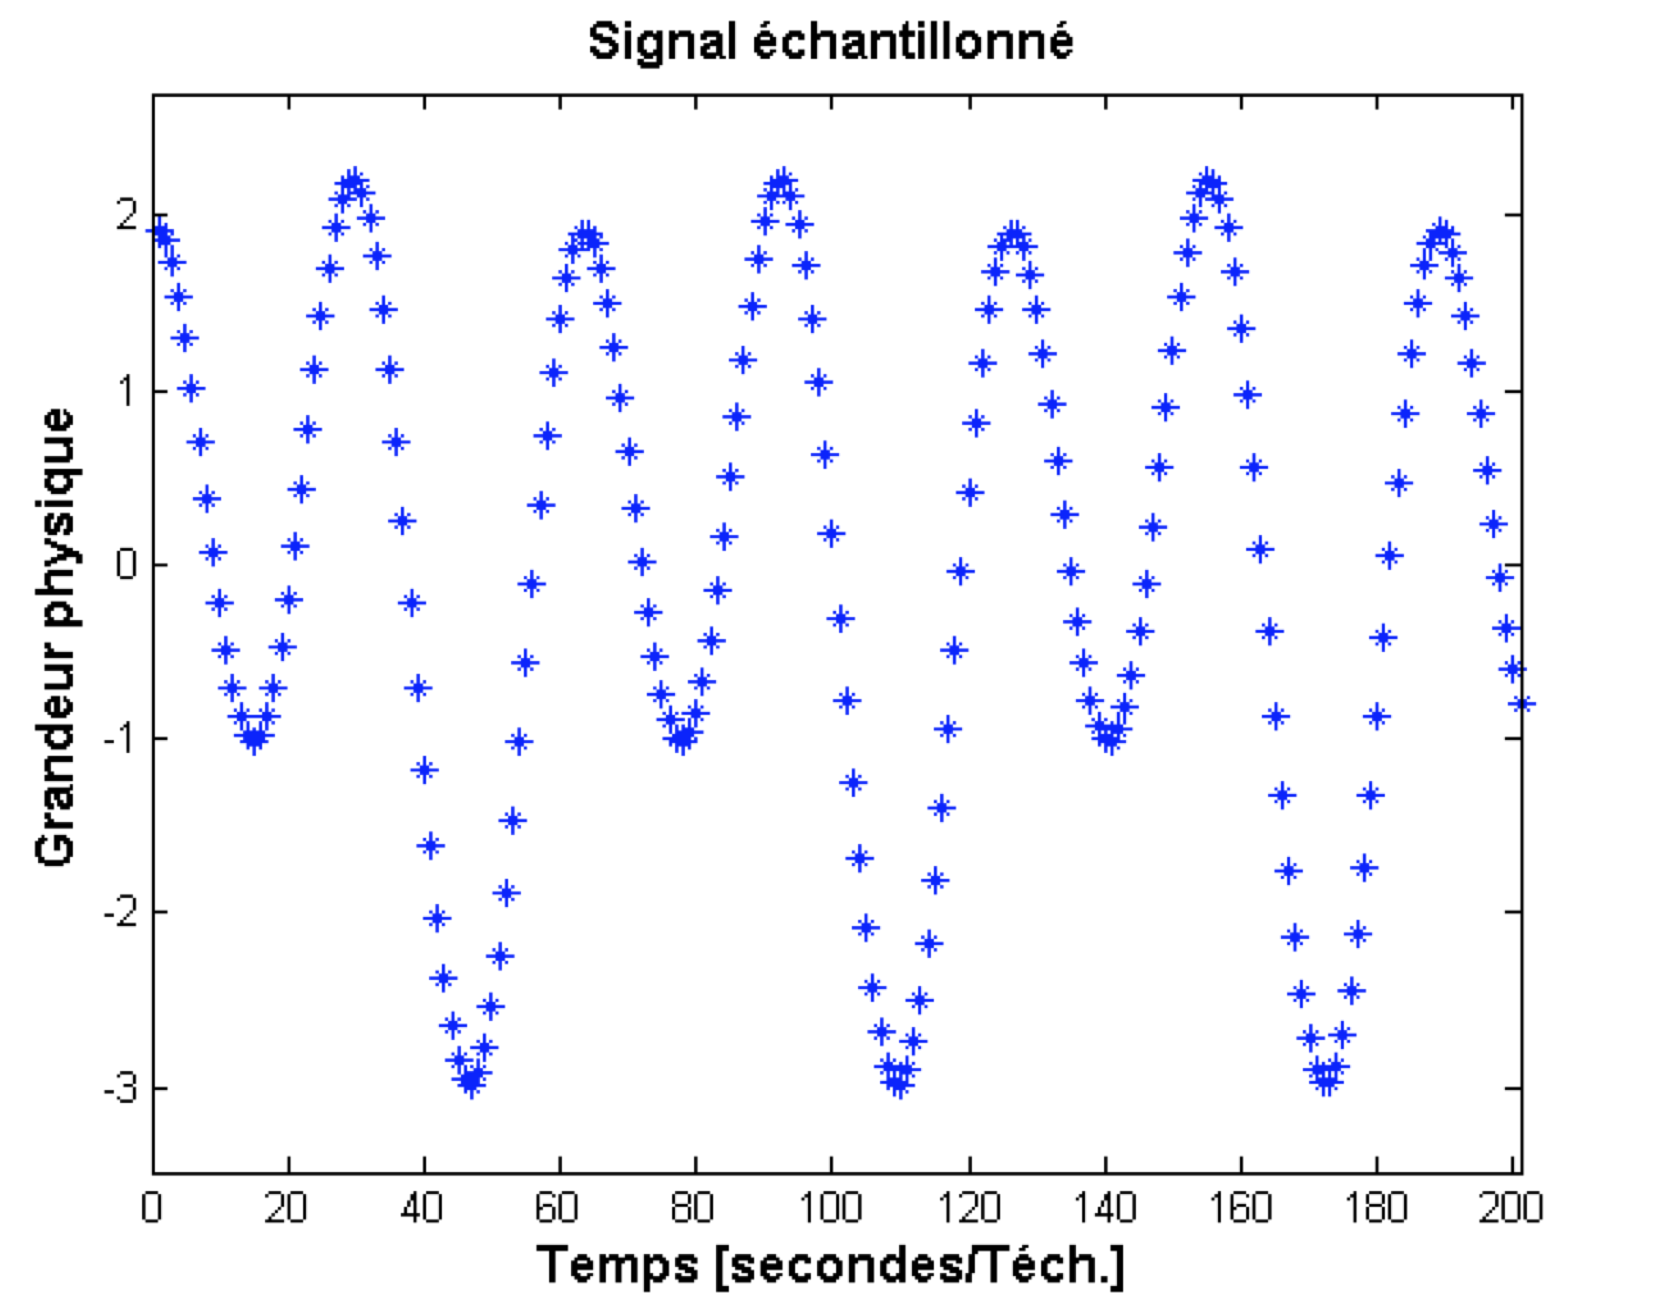
\includegraphics[width=.8\textwidth]{images/ad_1.png}
\end{center}

\end{frame}

\begin{frame}{Conversion analogique-digital (3)}

\begin{center}
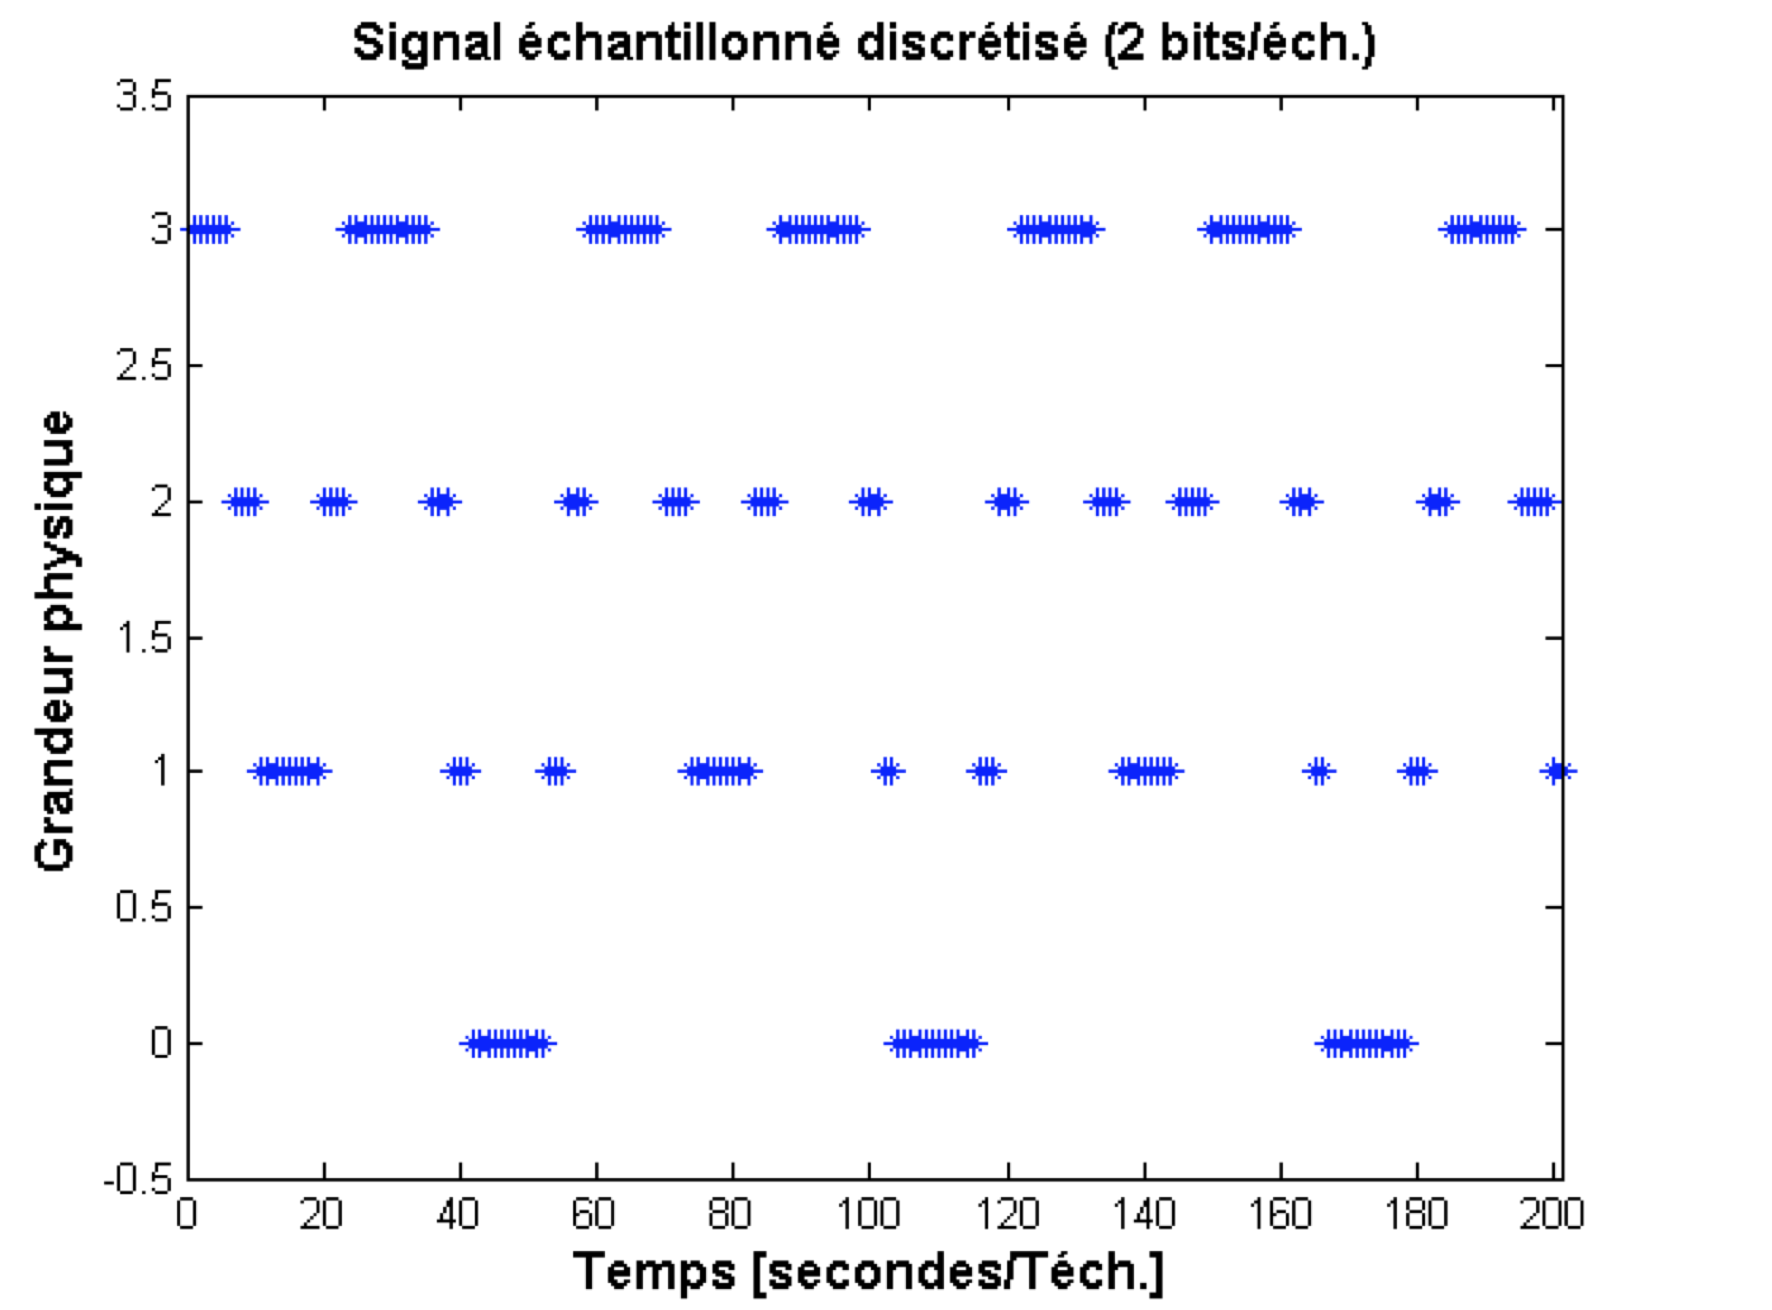
\includegraphics[width=.8\textwidth]{images/ad_2.png}
\end{center}

\end{frame}

\begin{frame}{Conversion analogique-digital (4)}

\begin{center}
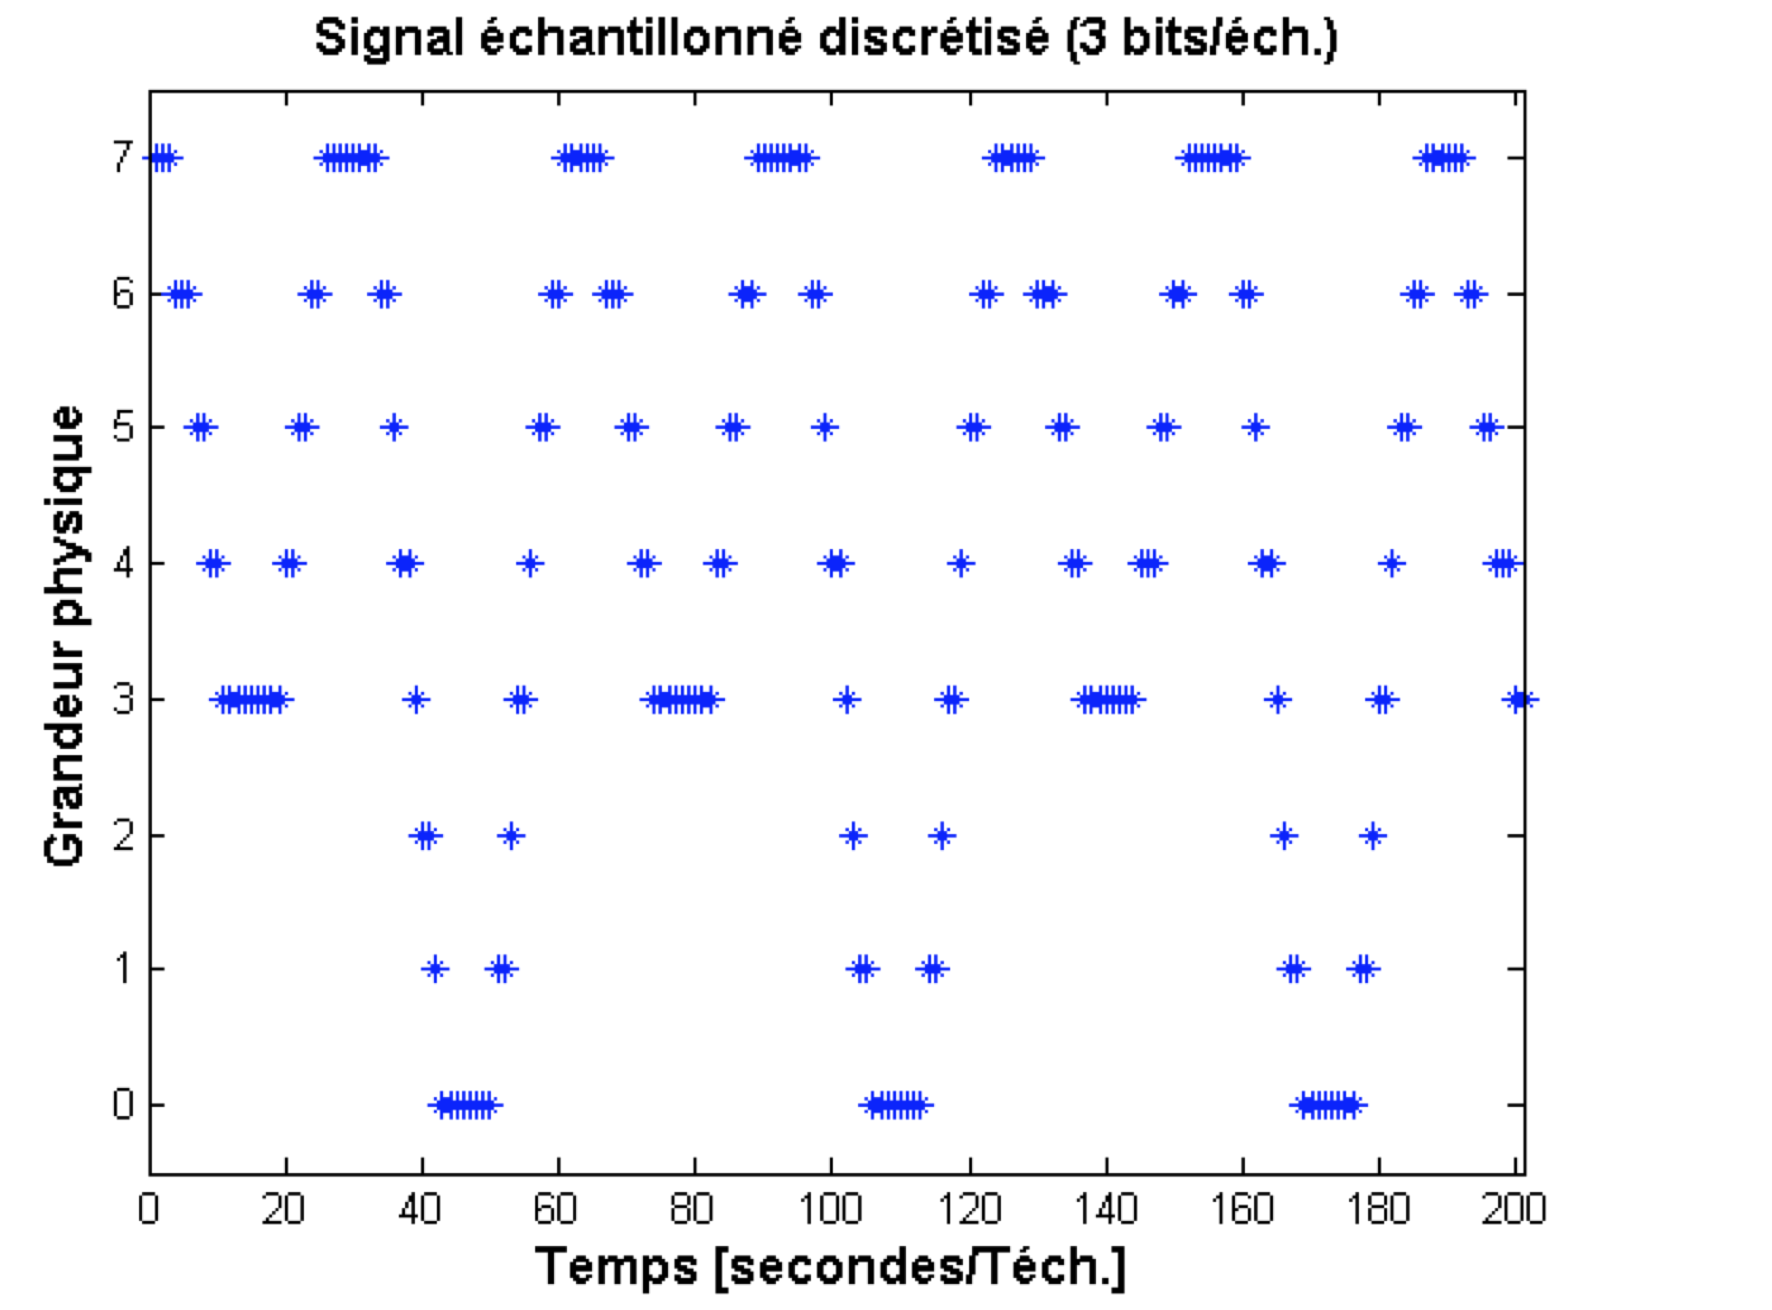
\includegraphics[width=.8\textwidth]{images/ad_3.png}
\end{center}

\end{frame}

\begin{frame}{Conversion analogique-digital (5)}

\begin{center}
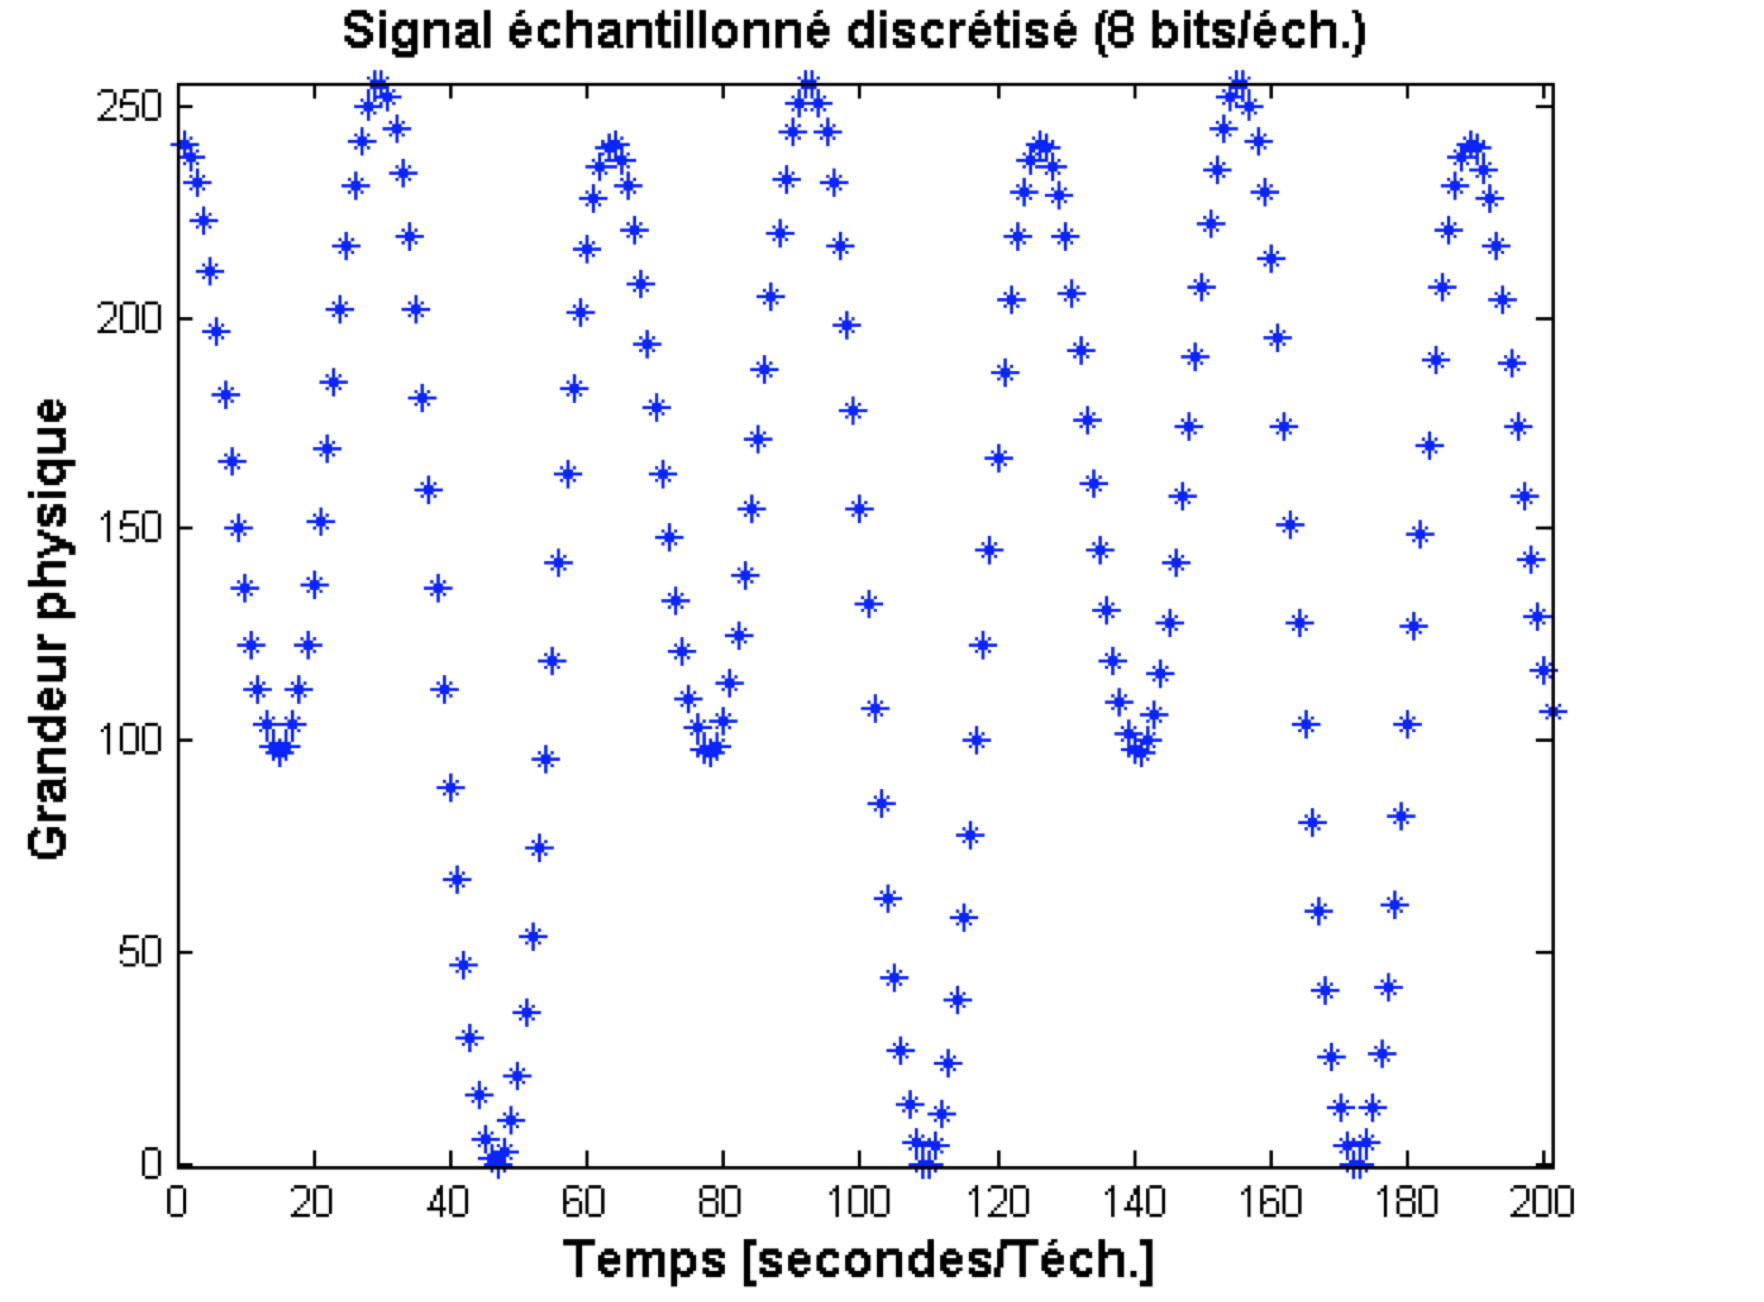
\includegraphics[width=.8\textwidth]{images/ad_4.png}
\end{center}

\end{frame}

\begin{frame}{Conversion analogique-digital : à retenir}

\begin{itemize}
\itemsep1pt\parskip0pt\parsep0pt
\item
  Deux fonctions utiles (pour le moment)

  \begin{itemize}
  \itemsep1pt\parskip0pt\parsep0pt
  \item
    void ADC\_Init(void)
  \item
    unsigned char getVoltage(void)
  \end{itemize}
\end{itemize}

\end{frame}

\section{Interruptions}\label{interruptions}

\begin{frame}{Interruptions}

\begin{itemize}
\itemsep1pt\parskip0pt\parsep0pt
\item
  Rappels

  \begin{itemize}
  \itemsep1pt\parskip0pt\parsep0pt
  \item
    Une demande d'interruption est émise pas un des modules
    périphériques via la mémoire.
  \item
    Si cette interruption est acceptée par notre configuration
    (interruption en général et interruption particulière), le code de
    l'interruption est exécuté.
  \item
    À la fin de cette exécution, le programme continue exactement où il
    se trouvait avant l'interruption.
  \item
    La demande d'interruption doit être effacée manuellement par routine
    d'interruption elle-même.
  \end{itemize}
\end{itemize}

\end{frame}

\begin{frame}{Interruptions : Fonctions}

\begin{itemize}
\itemsep1pt\parskip0pt\parsep0pt
\item
  void interruptEnable(void)
\item
  void interruptDisable(void)
\item
  void buttonInterruptEnable(void)
\item
  void buttonInterruptDisable(void)
\item
  void clearButtonInterruptRequest(void)
\end{itemize}

\end{frame}

\section{Timers}\label{timers}

\begin{frame}{Timers : fonctionnement}

\begin{center}
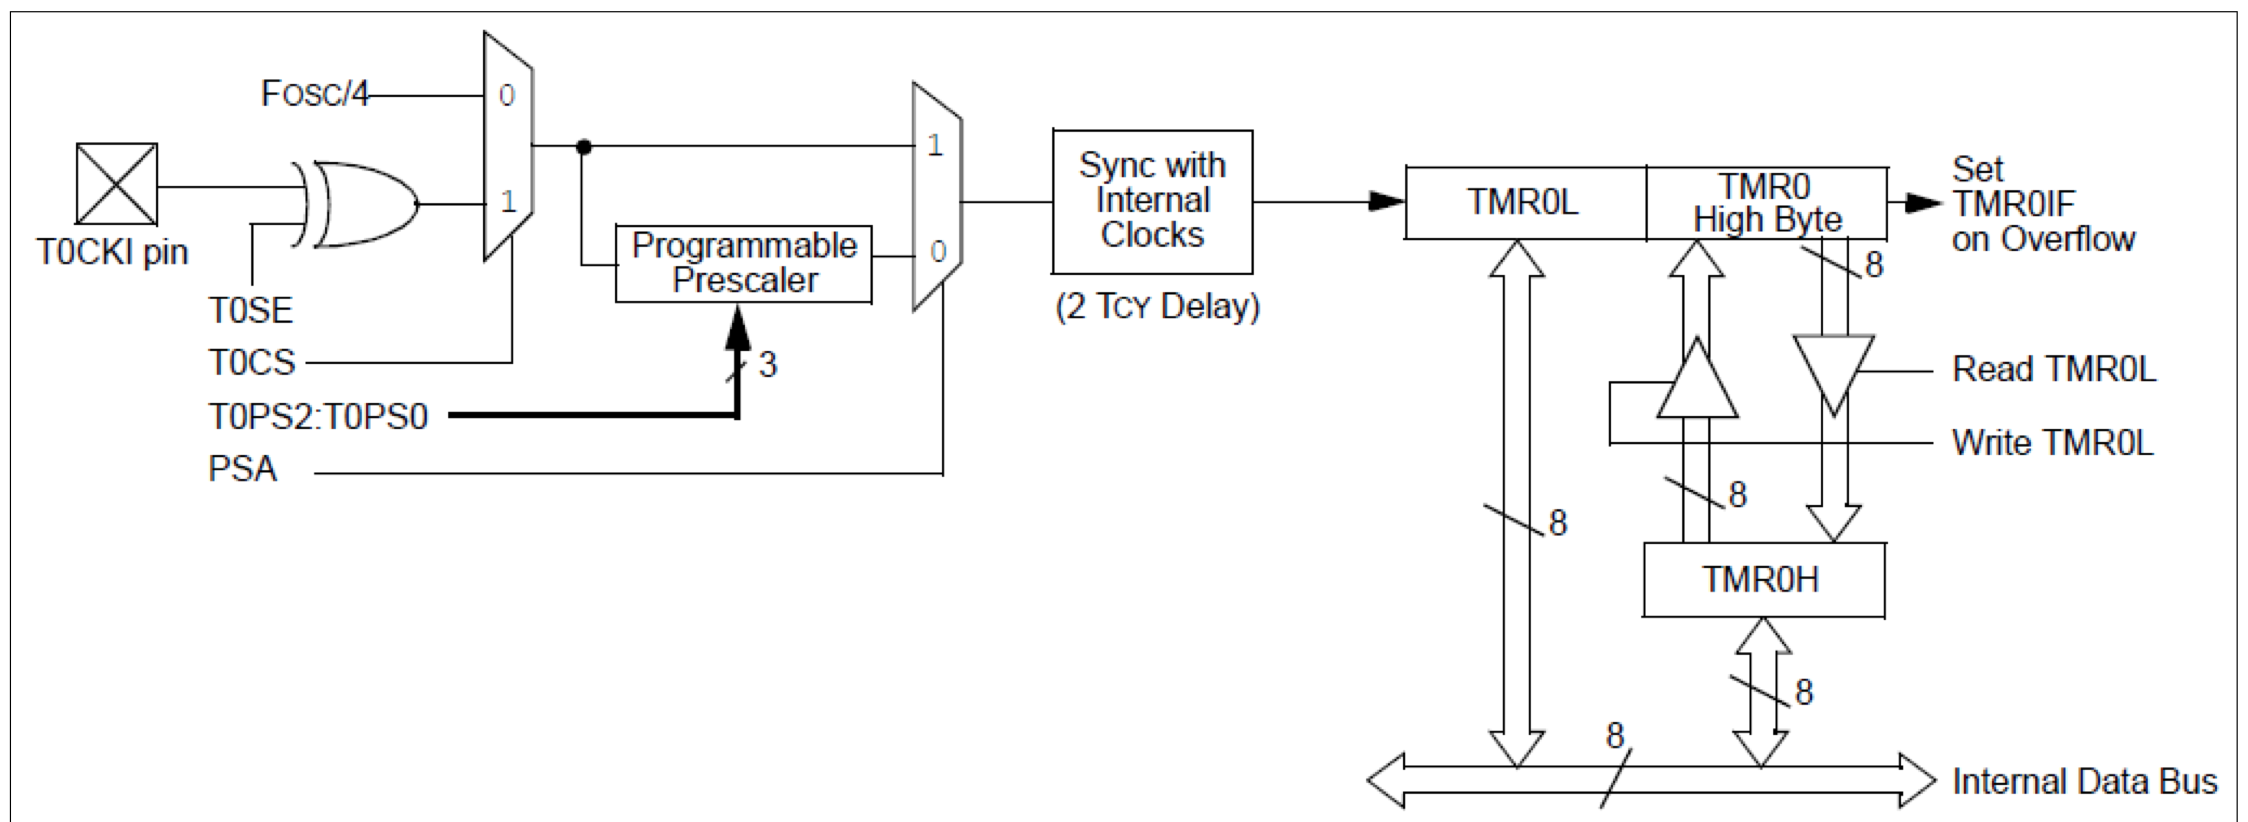
\includegraphics[width=1\textwidth]{images/tmr0.png}
\end{center}

\end{frame}

\begin{frame}{Timers : Fonctions}

\begin{itemize}
\itemsep1pt\parskip0pt\parsep0pt
\item
  initTimer(unisgned char preDivision, unsigned char priority)
  preDivision :

  \begin{itemize}
  \itemsep1pt\parskip0pt\parsep0pt
  \item
    111 = 1:256
  \item
    110 = 1:128
  \item
    101 = 1:64
  \item
    100 = 1:32
  \item
    011 = 1:16
  \item
    010 = 1:8
  \item
    001 = 1:4
  \item
    000 = 1:2
  \end{itemize}
\item
  void timerInterruptEnable(void)
\item
  void timerInterruptDisable(void)
\item
  void clearTimerInterruptRequest(void)
\end{itemize}

\end{frame}
